\section*{Dati e risultati}

\subsection*{Diodo 1N4007}

Per studiare la caratteristica $I-V$ (corrente-tensione) di un diodo 1N4007 sia in polarizzazione inversa che in diretta ci siamo mossi come segue: abbiamo collegato il diodo all'alimentatore di tensione continua, misurando con il multimetro la corrente assorbita dal diodo.
Ricordiamo che durante questa prima fase dell'esperienza abbiamo prestato attenzione che la corrente attraversante il diodo non superasse i $700\,\si{\milli\ampere}$.
Grazie ai dati misurati abbiamo graficato la curva caratteristica $I-V$ del diodo, mostrata in figura \ref{fig:diodo}.

%\begin{SCfigure}[1][b!]
\begin{SCfigure}
    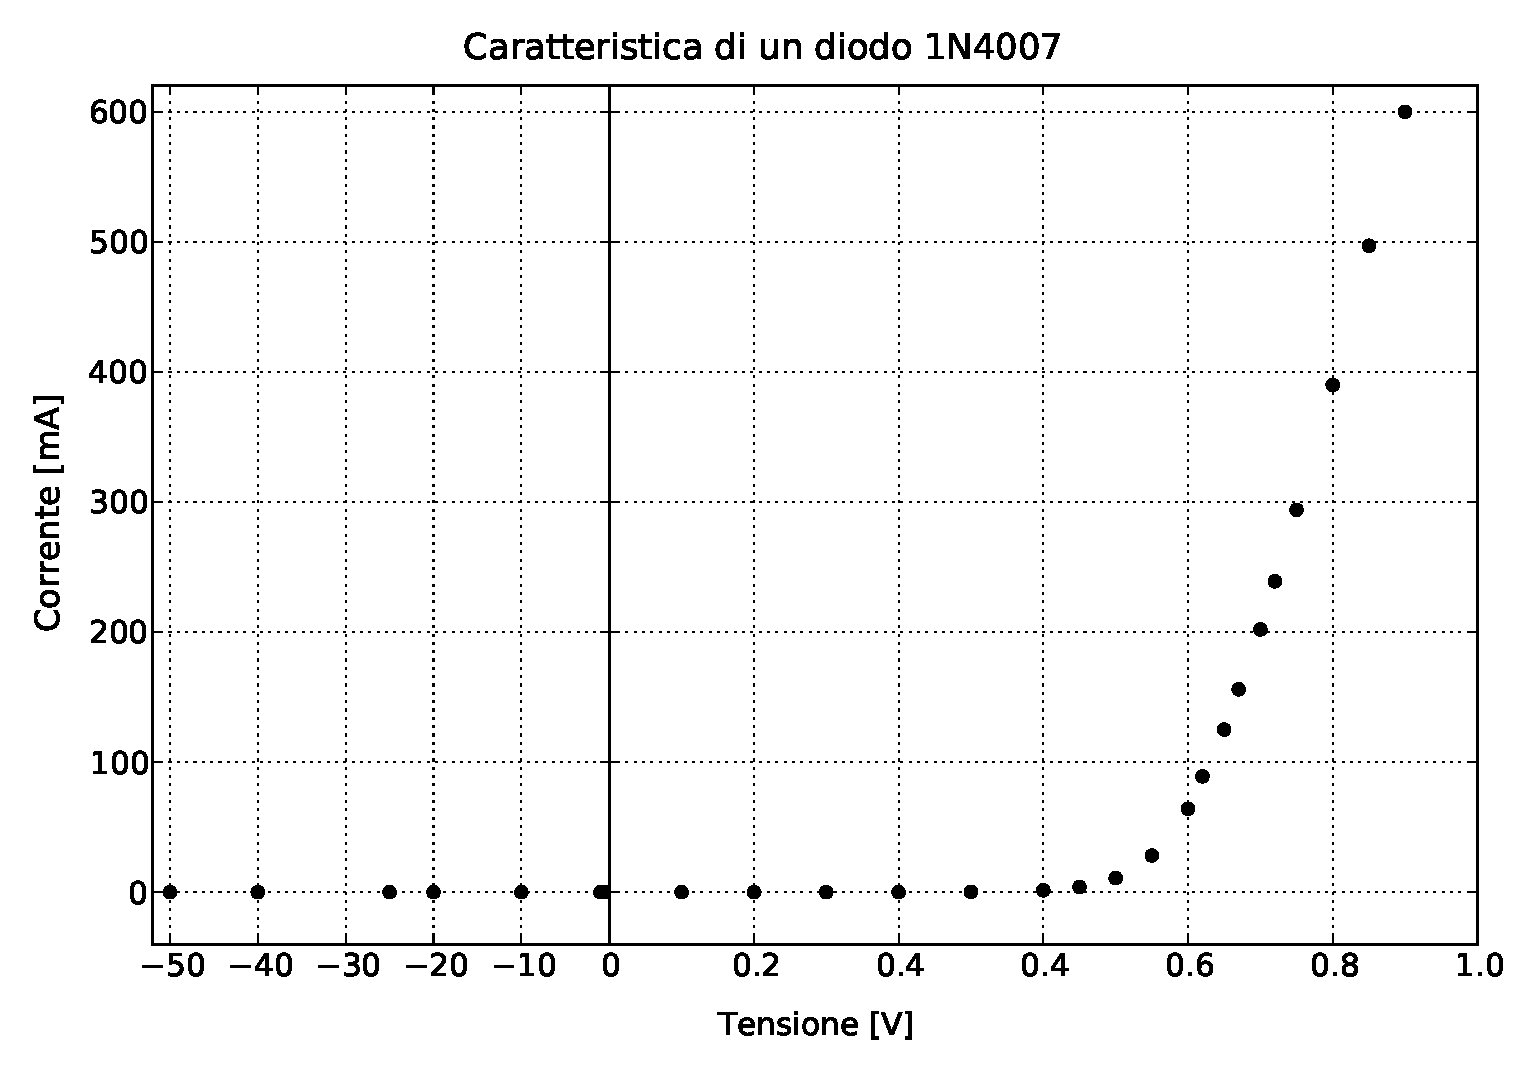
\includegraphics[scale=0.50]{diodo.pdf}
    \caption{La figura mostra la caratteristica corrente-tensione ($I-V$) di un diodo 1N4007. Questo tipo di diodi ha una tensione di breakdown di circa 1000 V, valori che con il nostro alimentatore non siamo in grado di raggiungere.
    La corrente di leakage è praticamente inesistente, mentre la tensione di cut-in è di circa 0.5 V, valore vicino al valore tipico di 0.6 V dei diodi al silicio. }
    \label{fig:diodo}
\end{SCfigure}
%\end{SCfigure}

\subsection*{Cella fotovoltaica}

Come secondo obbiettivo abbiamo valutato la caratteristica $I-V$ di una cella fotovoltaica monocristallina al silicio. Questo andamento è stato valutato sia ponendo la cella fotovoltaica al buio, ovvero ponendola all'interno del proprio involucro di cartone, sia esponendola ad una sorgente luminosa.
Come nel caso precedente abbiamo misurato mediante il multimetro la correte passante nella cella fotovoltaica pe poi studiane l'andamento in funzione della tensione.
Anche in questo caso abbiamo dovuto fare attenzione che la corrente massima nella cella fotovoltaica non superasse i $100\,\si{\milli\ampere}$.

\begin{SCfigure}
    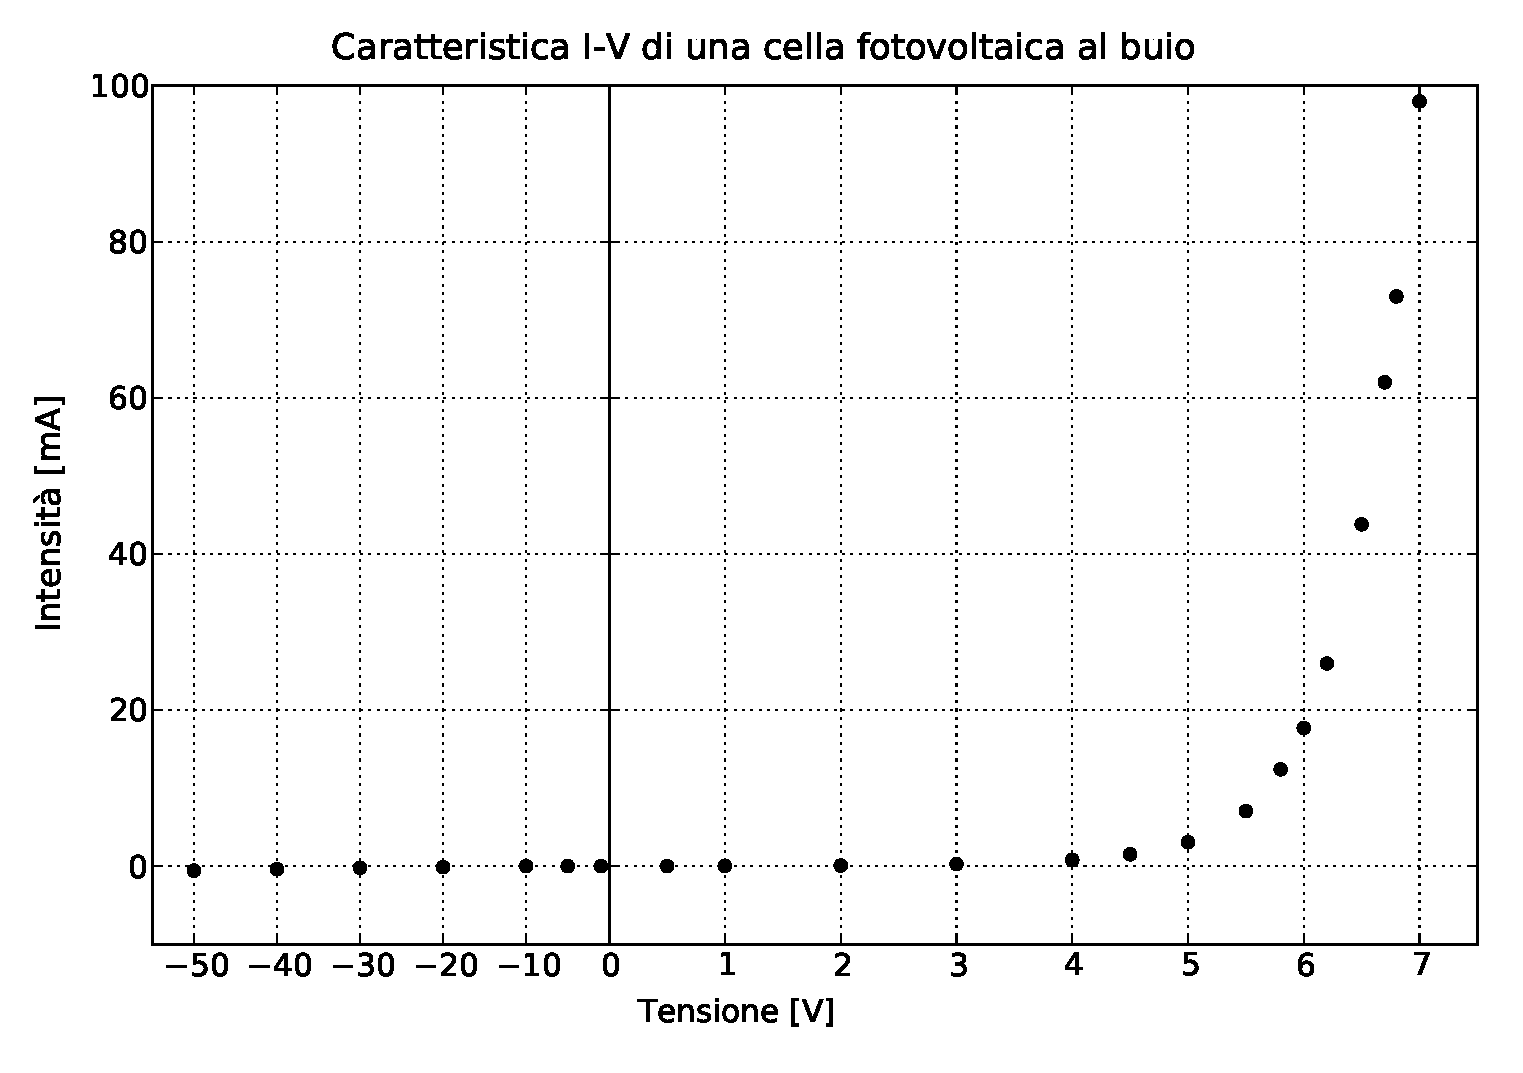
\includegraphics[scale=0.5]{buio.pdf}
    \caption{La caratteristica I-V di una cella fotovoltaica monocristallina al silicio al buio è per molti aspetti simile alla caratteristica di un diodo, con la differenza che la tensione di attivazione è di circa 5 V.}
    \label{fig:buio}
\end{SCfigure}

\begin{SCfigure}
    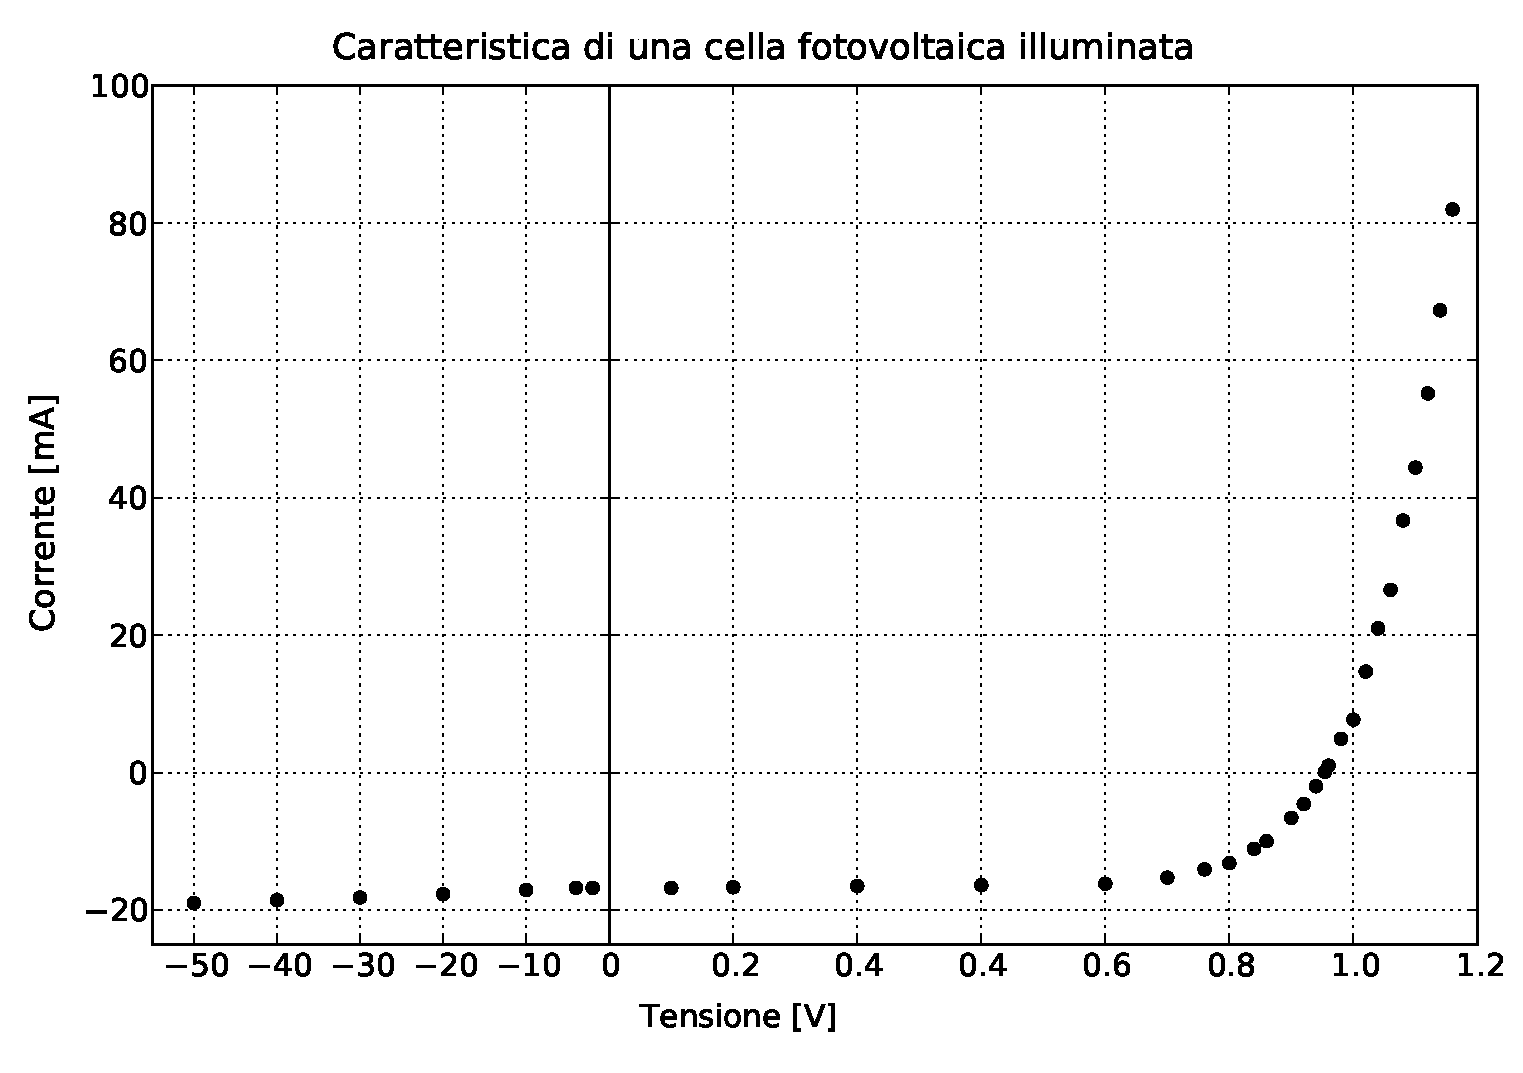
\includegraphics[scale=0.5]{luce.pdf}
    \caption{Questo grafico ilustra la carateristica $I-V$ di una cella fotovoltaica al silicio esposta ad una sorgente luminosa. Sotto queste condizioni, la curva caratteristica varia.}
    \label{fig:luce}
\end{SCfigure}

Infine abbiamo calcolato il FillFactor. Il rapporto tra il prodotto $I_m$ e $V_m$ (rispettivamente i valori di intensità di corrente e tensione il cui rapporto è massimo e quindi la potenza ottenibile dalla cella è massima, ossia in corrispondenza del ginocchio della curva) e il prodotto tra $I\ped{sc}$ e $V\ped{oc}$ (che indicano rispettivamente la corrente di corto circuito per la tensione a vuoto) è chiamato appunto FillFactor o fattore di riempimento della cella.
Il FillFactor dà un’indicazione delle prestazioni della cella.
Quest’ultimo nelle celle al silicio cristallino assume valori generalmente intorno a 0,75 e 0,80. Il FillFactor è anche un parametro di giudizio sul rendimento della cella: elevati valori di questi parametri sono anche indicatori di migliori prestazioni.

\begin{equation}
	\text{FillFactor} \,=\, \frac{I_m\,*\,V_m}{I\ped{sc}\,*\,V\ped{oc}} \,=\, ...
\end{equation}

